\section{Displacement observables}
\label{sec:displacement}

Every result in this report is expressed as a function of \emph{how displaced}
a shower is. We therefore begin by defining the displacement observables and,
crucially, by explaining how they are obtained for reconstructed objects that
carry no truth information.

\subsection{Definitions}

\begin{figure}[!htbp]
  \centering
  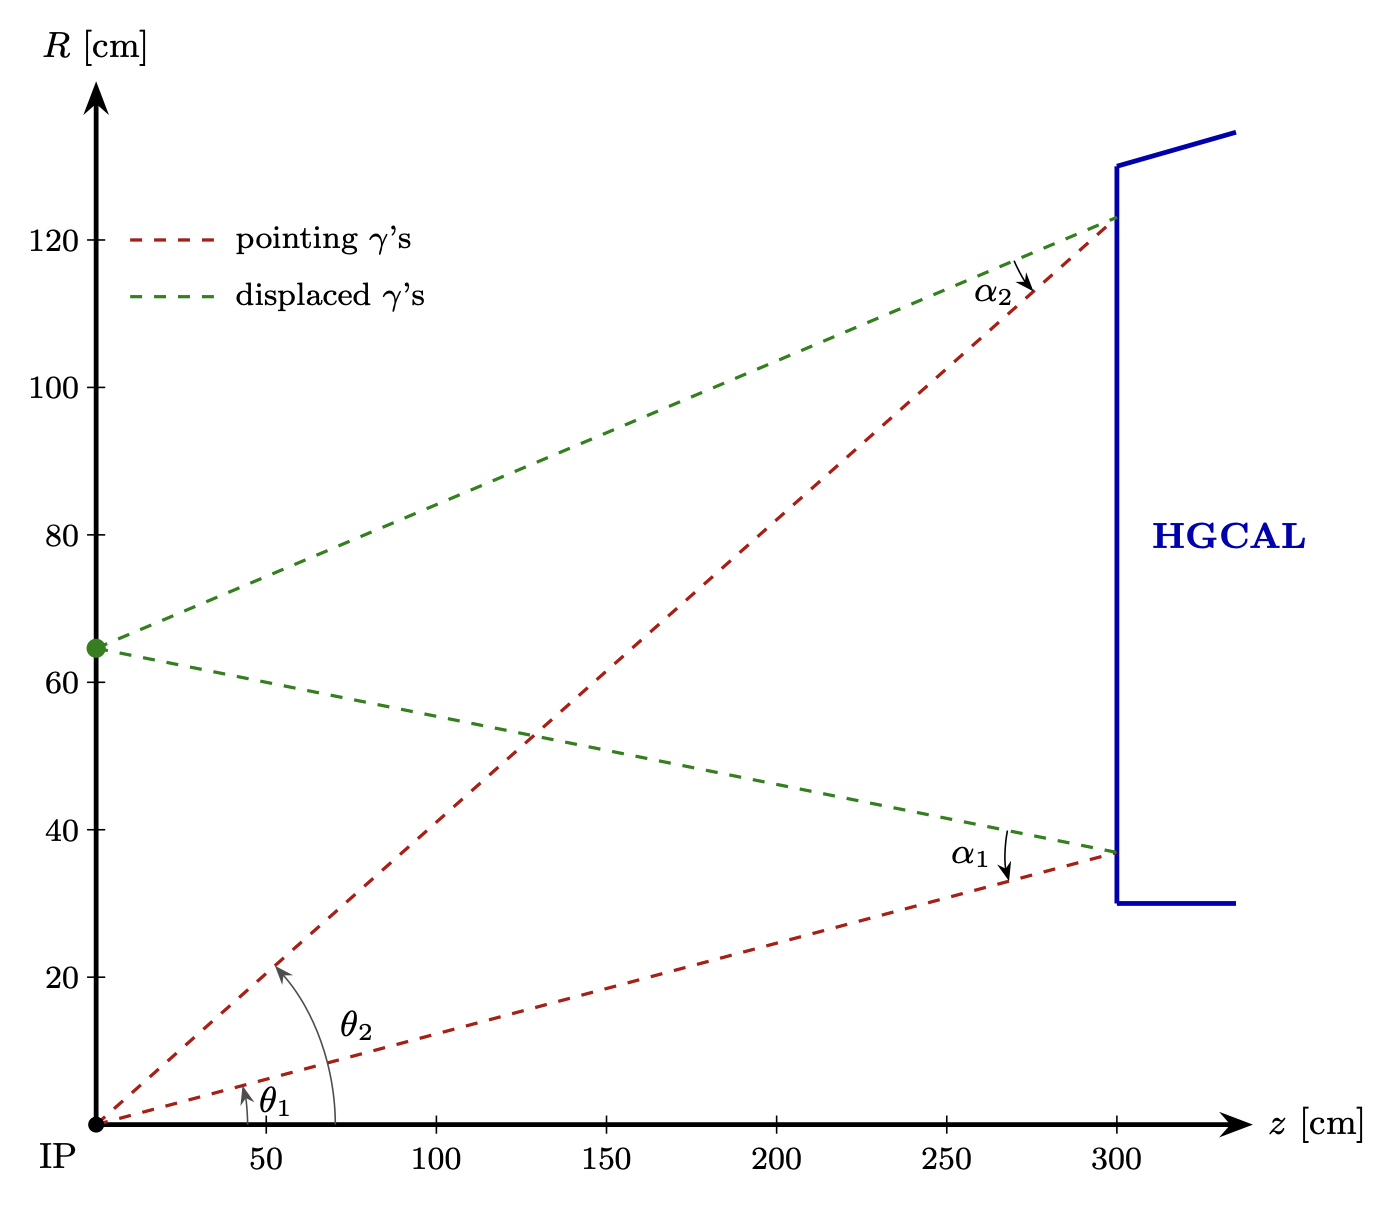
\includegraphics[width=\linewidth]{figures/hgcal_nonpointing.png}
  \caption{Displacement geometry in the $(z,R)$ plane. Pointing photons (red)
  travel radially from the interaction point (IP) and reach the HGCAL front face
  at a polar angle $\theta$ with non-pointing angle $\alphainc=0$. Displaced
  photons (green) originate at a transverse distance $\R$ from the beamline at
  $z=0$ and strike the calorimeter with $\alphainc>0$; two displaced trajectories
  from the same vertex illustrate that a single $\R$ can correspond to different
  incidence angles $\alphainc$.}
  \label{fig:geometry}
\end{figure}

Consider a photon that is created at a production vertex
$\mathbf{x}_v=(x_v,y_v,z_v)$ and travels in a straight line to the HGCAL front
face, located at $z\simeq\SI{321}{cm}$ from the interaction
point (Fig.~\ref{fig:geometry}). We characterize its displacement by two
quantities:
\begin{itemize}
  \item the \textbf{displacement radius} \R{}, defined as the transverse
  distance from the beamline at which the photon's extrapolated trajectory crosses the plane
  $z=0$,
  \begin{equation}
    \R = \sqrt{x_0^2 + y_0^2}\,,
    \label{eq:Rdef}
  \end{equation}
  where $(x_0,y_0)$ is the trajectory back-projected to $z=0$;
  \item the \textbf{non-pointing angle} \alphainc{}, the angle between the
  photon's momentum $\mathbf{p}$ and its position vector at the HGCAL face,
  i.e.\ the line joining the interaction point to the impact point
  $\mathbf{x}_{\text{face}}$,
  \begin{equation}
    \alphainc = \arccos\!\left(
      \frac{\mathbf{x}_{\text{face}}\cdot\mathbf{p}}
           {\lvert\mathbf{x}_{\text{face}}\rvert\,\lvert\mathbf{p}\rvert}
    \right).
    \label{eq:alphadef}
  \end{equation}
  A prompt, pointing photon travels radially, so
  $\mathbf{x}_{\text{hit}}\parallel\mathbf{p}$ and $\R=\alphainc=0$; a displaced
  photon has $\R>0$ and $\alphainc>0$.
\end{itemize}
It is also useful to introduce the polar angle $\theta$ between the photon
momentum and the beam axis, with $\tan\theta = p_T/|p_z|$. As shown in
Fig.~\ref{fig:geometry}, \alphainc{} rather than \R{} is the more fundamental driver of the clustering
behaviour, but \R{} has a direct geometric interpretation as the transverse distance, so both are retained throughout.

For a \emph{simulated} photon these quantities are trivial: the production
vertex and momentum are known from the generator, and \R{} follows from a
straight-line extrapolation. We verified this extrapolation numerically---the
displacement computed from the SimTrackster's SimTrack reproduces the generator-level value, and pointing photons correctly yield
$\R,\alphainc\approx0$.

\subsection{Reconstructing the displacement}

The difficulty lies on the reconstruction side. A reconstructed Trackster has no
production vertex, and it does not need to correspond one-to-one to a SimTrackster: it
may contain only a fragment of a true shower, or it may span multiple showers.
Nonetheless, the fake-, duplicate- and merge-rate metrics defined below require a
displacement value in order to place each Trackster in a histogram bin. We therefore reconstruct \R{} directly from the
Trackster geometry.

Each Trackster provides an energy-weighted barycentre
$\mathbf{x}_c=(x_c,y_c,z_c)$ and a principal-axis direction
$\mathbf{u}=(u_x,u_y,u_z)$ obtained from a principal-component analysis (PCA) of
its LayerClusters. Treating the shower as a straight line through
$\mathbf{x}_c$ along $\mathbf{u}$ and extrapolating to $z=0$ gives
\begin{align}
  x_0 &= x_c - z_c\,\frac{u_x}{u_z}\,, &
  y_0 &= y_c - z_c\,\frac{u_y}{u_z}\,,
  \label{eq:recoR}
\end{align}
and $\R_{\text{reco}}=\sqrt{x_0^2+y_0^2}$ from Eq.~\eqref{eq:Rdef}. Care is taken so that the extrapolation uses the
correct sign of $u_z$. This straight-line treatment is exact for photons, which
makes them the ideal probe for validating the method.

\subsection{Error budget and the choice of direction estimator}

\begin{figure*}[!tp]
  \centering
  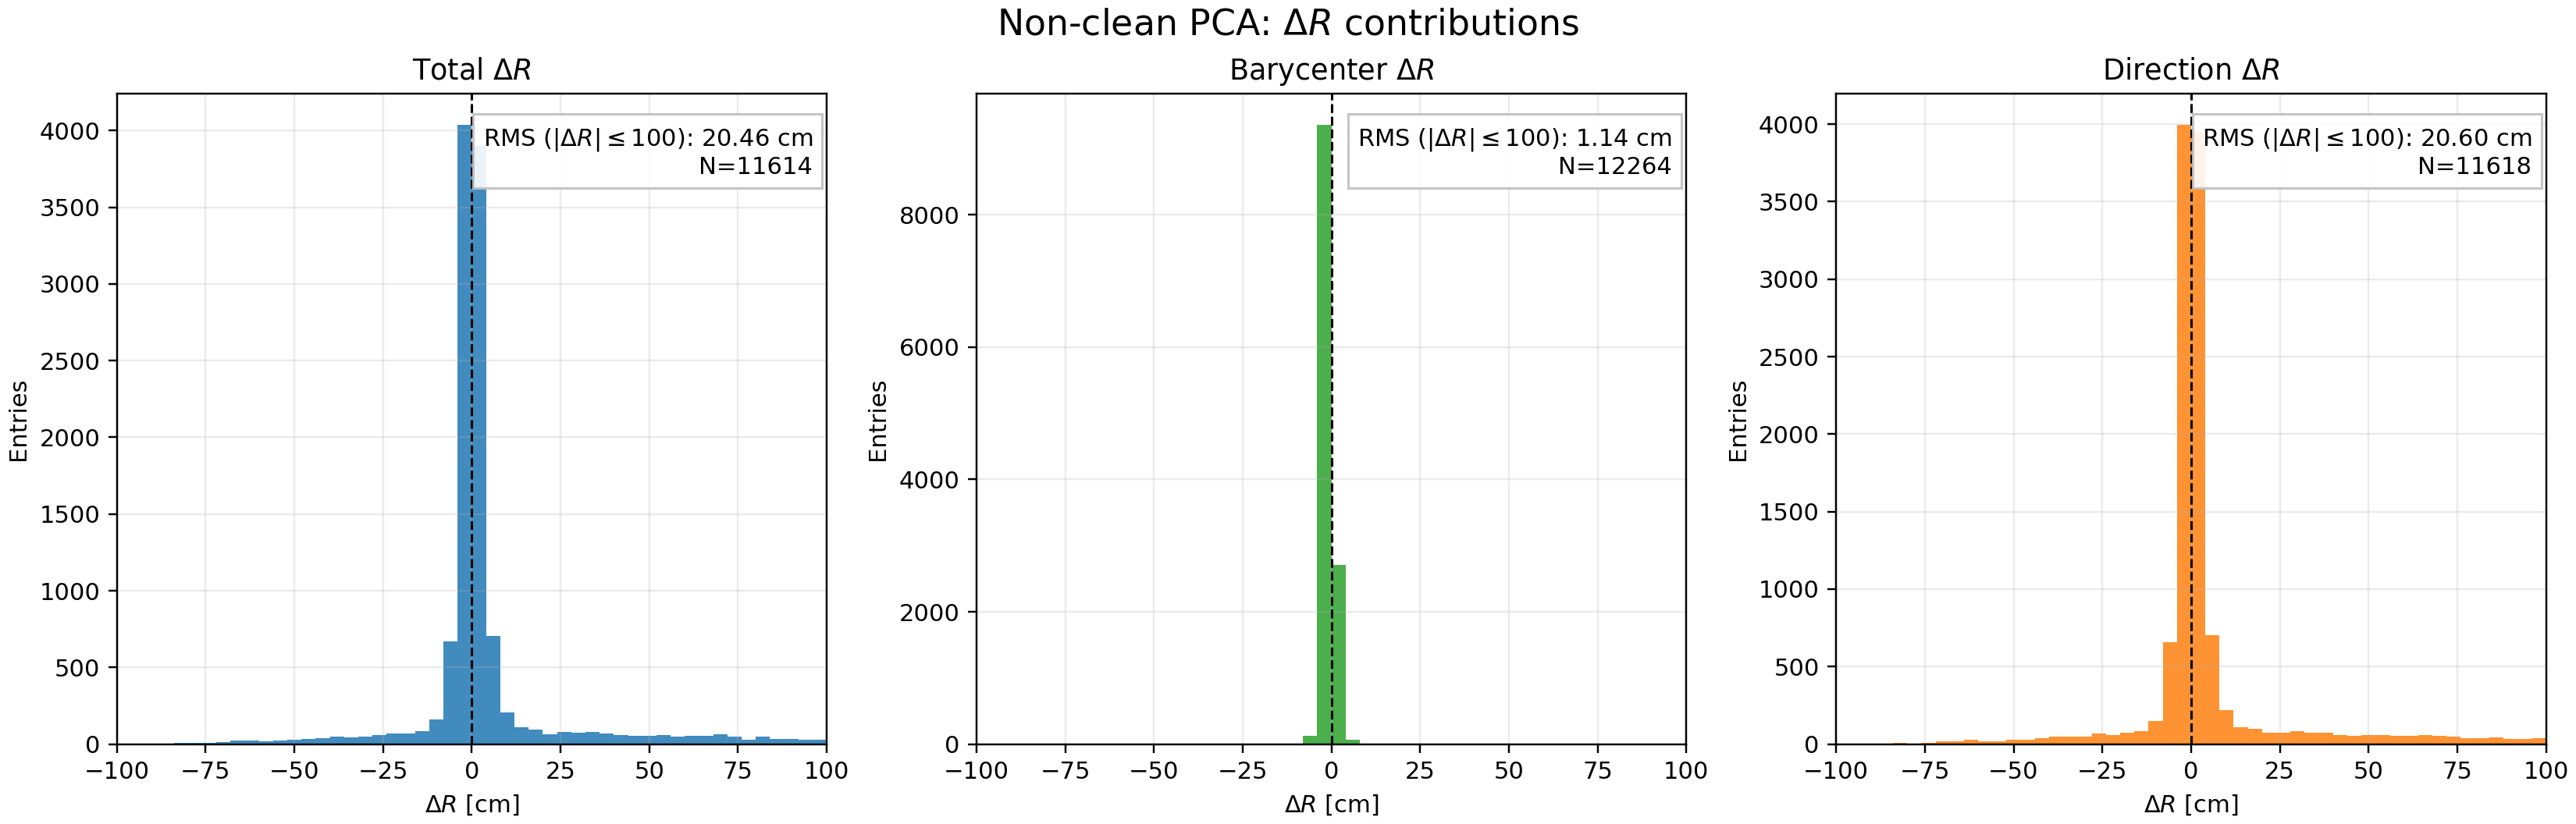
\includegraphics[width=0.88\textwidth]{figures/non_clean_pca_deltaR_contributions.png}
  \caption{Decomposition of the displacement-radius error into its two sources,
  for the default (ordinary) PCA. \emph{Left:} the full error
  $\Delta\R=\R_{\text{reco}}-\R_{\text{truth}}$
  ($\text{RMS}=\SI{20.46}{cm}$). \emph{Centre:} the error when only the
  barycentre is reconstructed and the true direction is used
  ($\text{RMS}=\SI{1.14}{cm}$). \emph{Right:} the error when only the direction
  is reconstructed and the true barycentre is used
  ($\text{RMS}=\SI{20.60}{cm}$). The direction term alone reproduces the full
  error, proving that the resolution budget is spent almost entirely on the
  shower direction.}
  \label{fig:decomp}
\end{figure*}

The accuracy of $\R_{\text{reco}}$ sets the resolution with which any reco-side
metric can be studied, so we characterized its error in detail. We quantify it by
\begin{equation}
  \Delta\R \equiv \R_{\text{reco}} - \R_{\text{truth}},
  \label{eq:deltaR}
\end{equation}
summarized throughout by its RMS. Our starting point was the direction estimator
that CMSSW already exposes: the ordinary PCA of \texttt{TrackstersPCA.cc}, which
builds the energy-weighted covariance matrix of the LayerCluster positions about
the barycentre, and makes the shower direction $\mathbf{u}$ to be its leading
eigenvector (the axis of largest spatial variance). Reusing this default out of
the box gave a broad error---$\text{RMS}(\Delta\R)\approx\SI{20}{cm}$ for the
sample of Fig.~\ref{fig:decomp}---and before trying to improve it we wanted to
know \emph{where} that error came from.

The error has only two possible sources, the barycentre $\mathbf{x}_c$ and the
direction $\mathbf{u}$, and they can be separated cleanly. We recompute
$\Delta\R$ twice: once with the reconstructed barycentre but the \emph{true}
direction (isolating the barycentre error), and once with the true barycentre but
the reconstructed direction (isolating the direction error). The answer is unambiguous (Fig.~\ref{fig:decomp}): the
barycentre alone contributes only $\text{RMS}(\Delta\R)=\SI{1.14}{cm}$, whereas
the direction alone contributes $\SI{20.60}{cm}$ and by itself reproduces the
$\SI{20.46}{cm}$ of the full error. The barycentre is essentially
perfect; the direction is entirely to blame. The reason is geometric: the
barycentre sits inside the shower and is well measured, but the small angular
uncertainty of $\mathbf{u}$ is amplified by the long
$z_c\sim\SI{320}{cm}$ over which Eq.~\eqref{eq:recoR} extrapolates back to $z=0$.
The same figure shows a systematic positive bias of order $+\SI{3}{cm}$,
consistent with \R{} being a positive-definite quantity.

Having localized the problem to the direction, we implemented and compared
several estimators of the shower axis. Each takes the LayerClusters (or RecHits)
of a Trackster and returns a unit direction:
\begin{itemize}
  \item \textbf{Ordinary PCA} (the CMSSW default): leading eigenvector of the
  energy-weighted covariance matrix
  $C=\sum_i w_i(\mathbf{x}_i-\mathbf{x}_c)(\mathbf{x}_i-\mathbf{x}_c)^{\!\top}$,
  where $\mathbf{x}_i$ and $w_i$ are the position and energy of LayerCluster $i$.
  It uses every LayerCluster, so secondary per-layer clusters and stray fragments
  can tilt the axis.
  \item \textbf{Clean PCA (10-to-10)}: the same eigenvector computation, but on a
  cleaned set that keeps only the single highest-energy LayerCluster in each
  layer, restricted to the ten layers before and the ten layers after the
  peak-energy layer. This suppresses the off-axis fragments that bias the
  covariance while retaining the well-measured shower core.
  \item \textbf{Endpoint layers}: the direction joining the barycentre of the
  first populated layer of the window to that of the last. It uses only the two
  extremes, so it is simple but sensitive to endpoint fluctuations.
  \item \textbf{Window barycentres}: per-layer energy-weighted barycentres are
  formed across the window and their trend in $z$ defines the axis, averaging out
  single-layer noise.
  \item \textbf{Weighted straight-line fit}: the shower is parametrized as a line
  $x(z)=x_0+(u_x/u_z)\,z$, $y(z)=y_0+(u_y/u_z)\,z$, and the slopes are obtained by
  minimizing the energy-weighted sum of squared transverse residuals of the
  LayerClusters to that line---a direct least-squares alternative to the PCA.
  \item \textbf{Weighted line fit with outlier refit}: the same fit, after which
  the $20\%$ of LayerClusters with the largest residuals are discarded and the
  line is refitted, reducing the pull of outliers; we tried this both on the
  $10$-to-$10$ window and over all layers.
  \item \textbf{RecHit PCA}: the covariance-eigenvector method applied to the raw
  RecHits instead of the LayerClusters, testing whether the finer granularity
  below the LayerCluster level helps.
\end{itemize}

\begin{figure*}[!tp]
  \centering
  \begin{subfigure}[t]{0.49\textwidth}
    \centering
    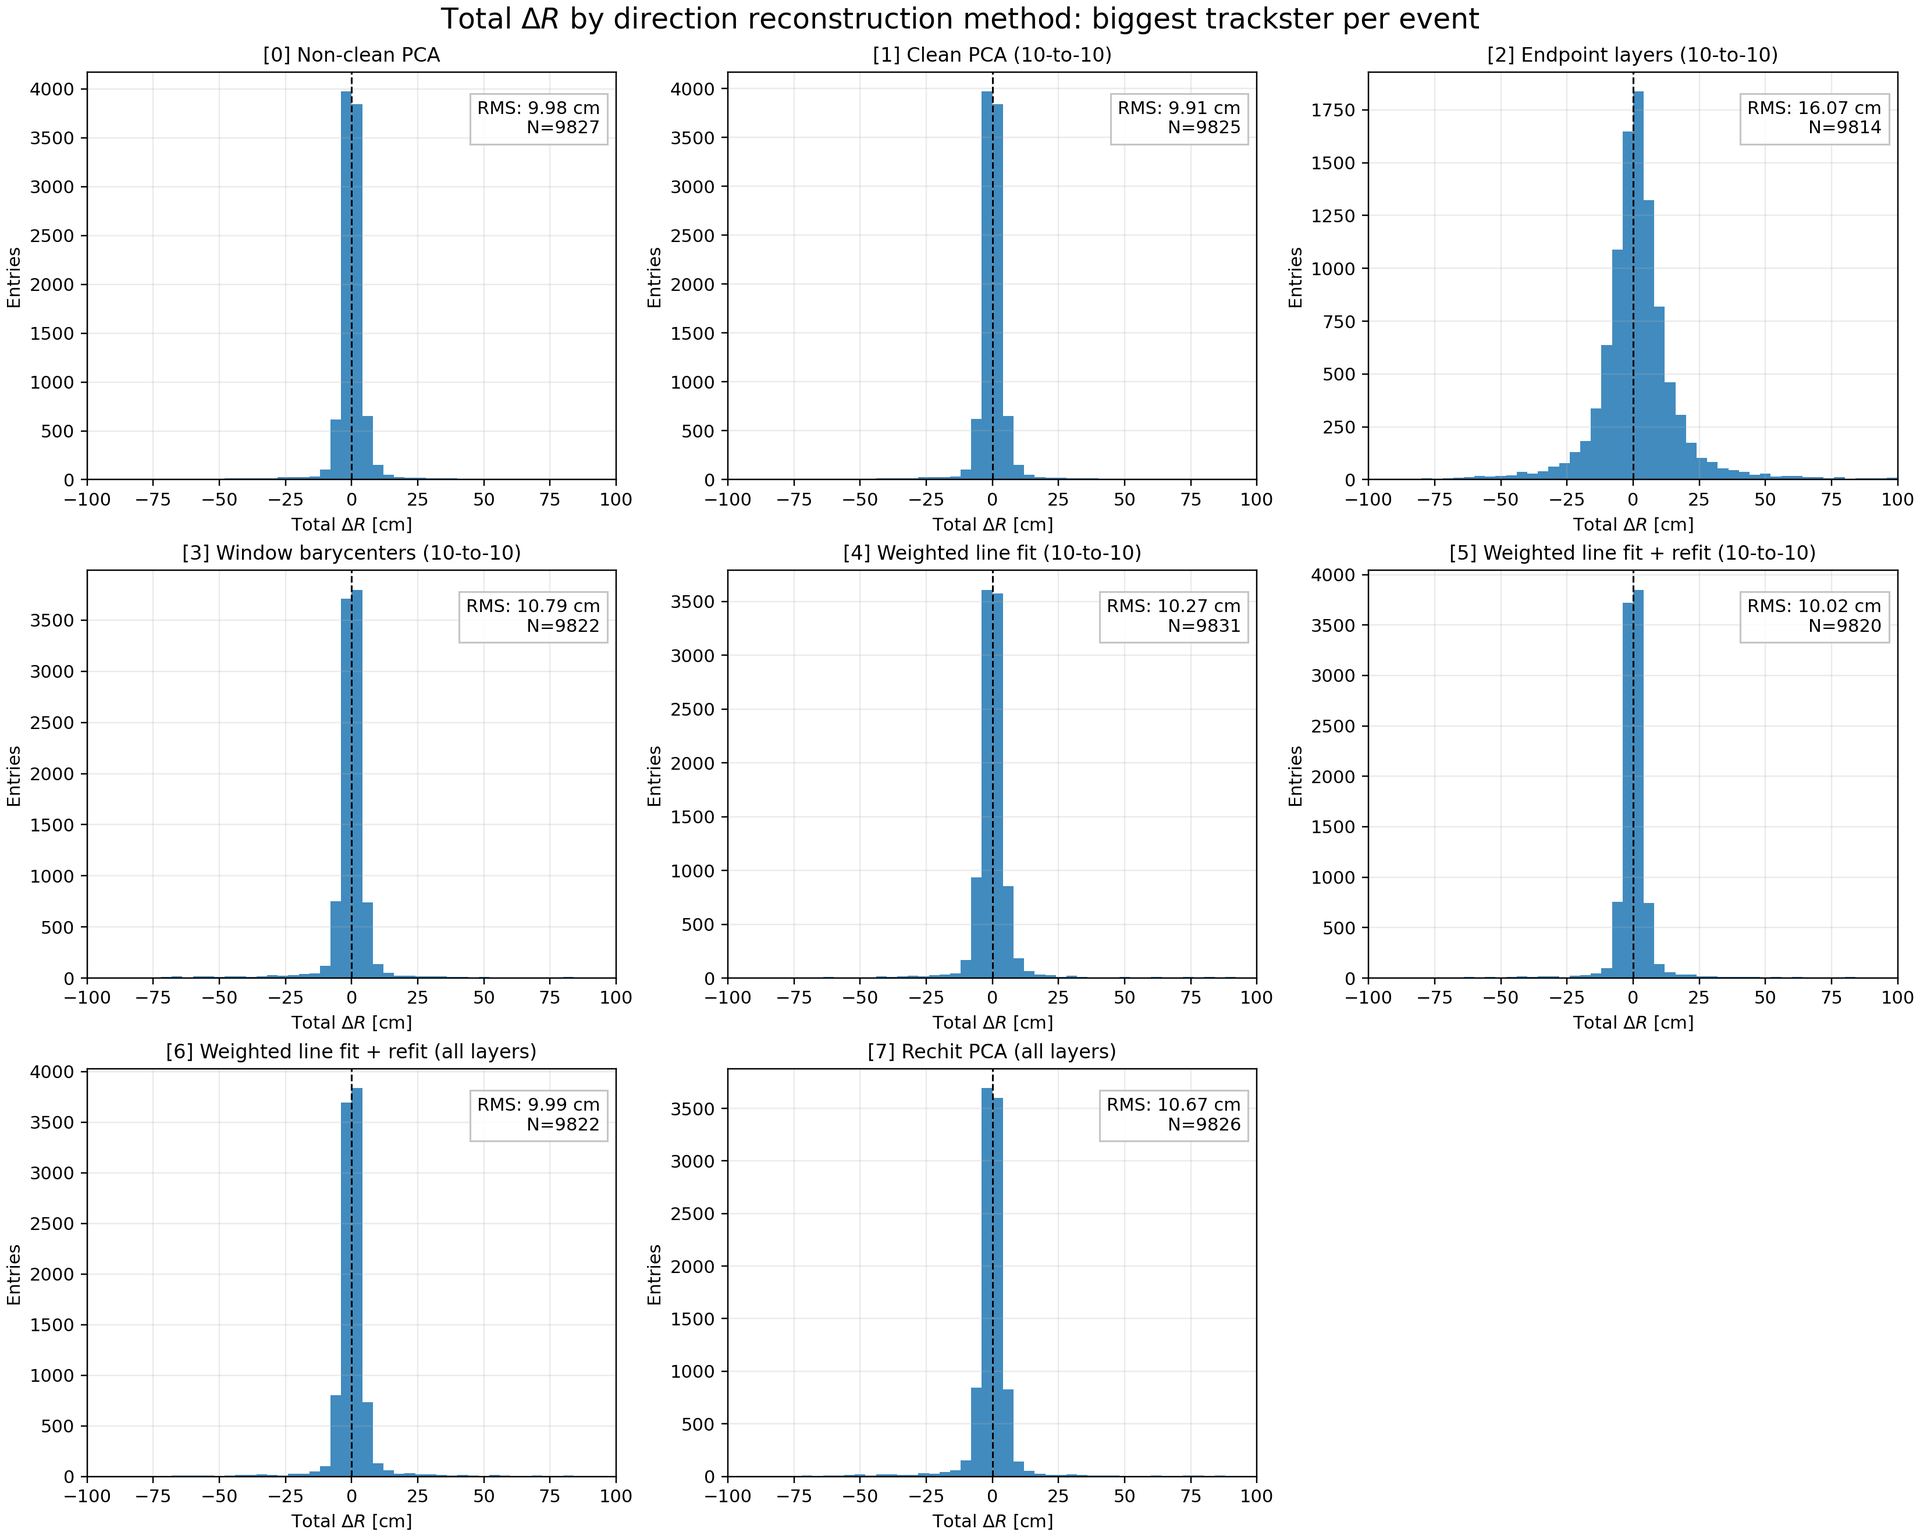
\includegraphics[width=\linewidth]{figures/r_resolution_methods_leading.png}
    \caption{leading (most energetic) Trackster per event}
    \label{fig:methods-lead}
  \end{subfigure}
  \hfill
  \begin{subfigure}[t]{0.49\textwidth}
    \centering
    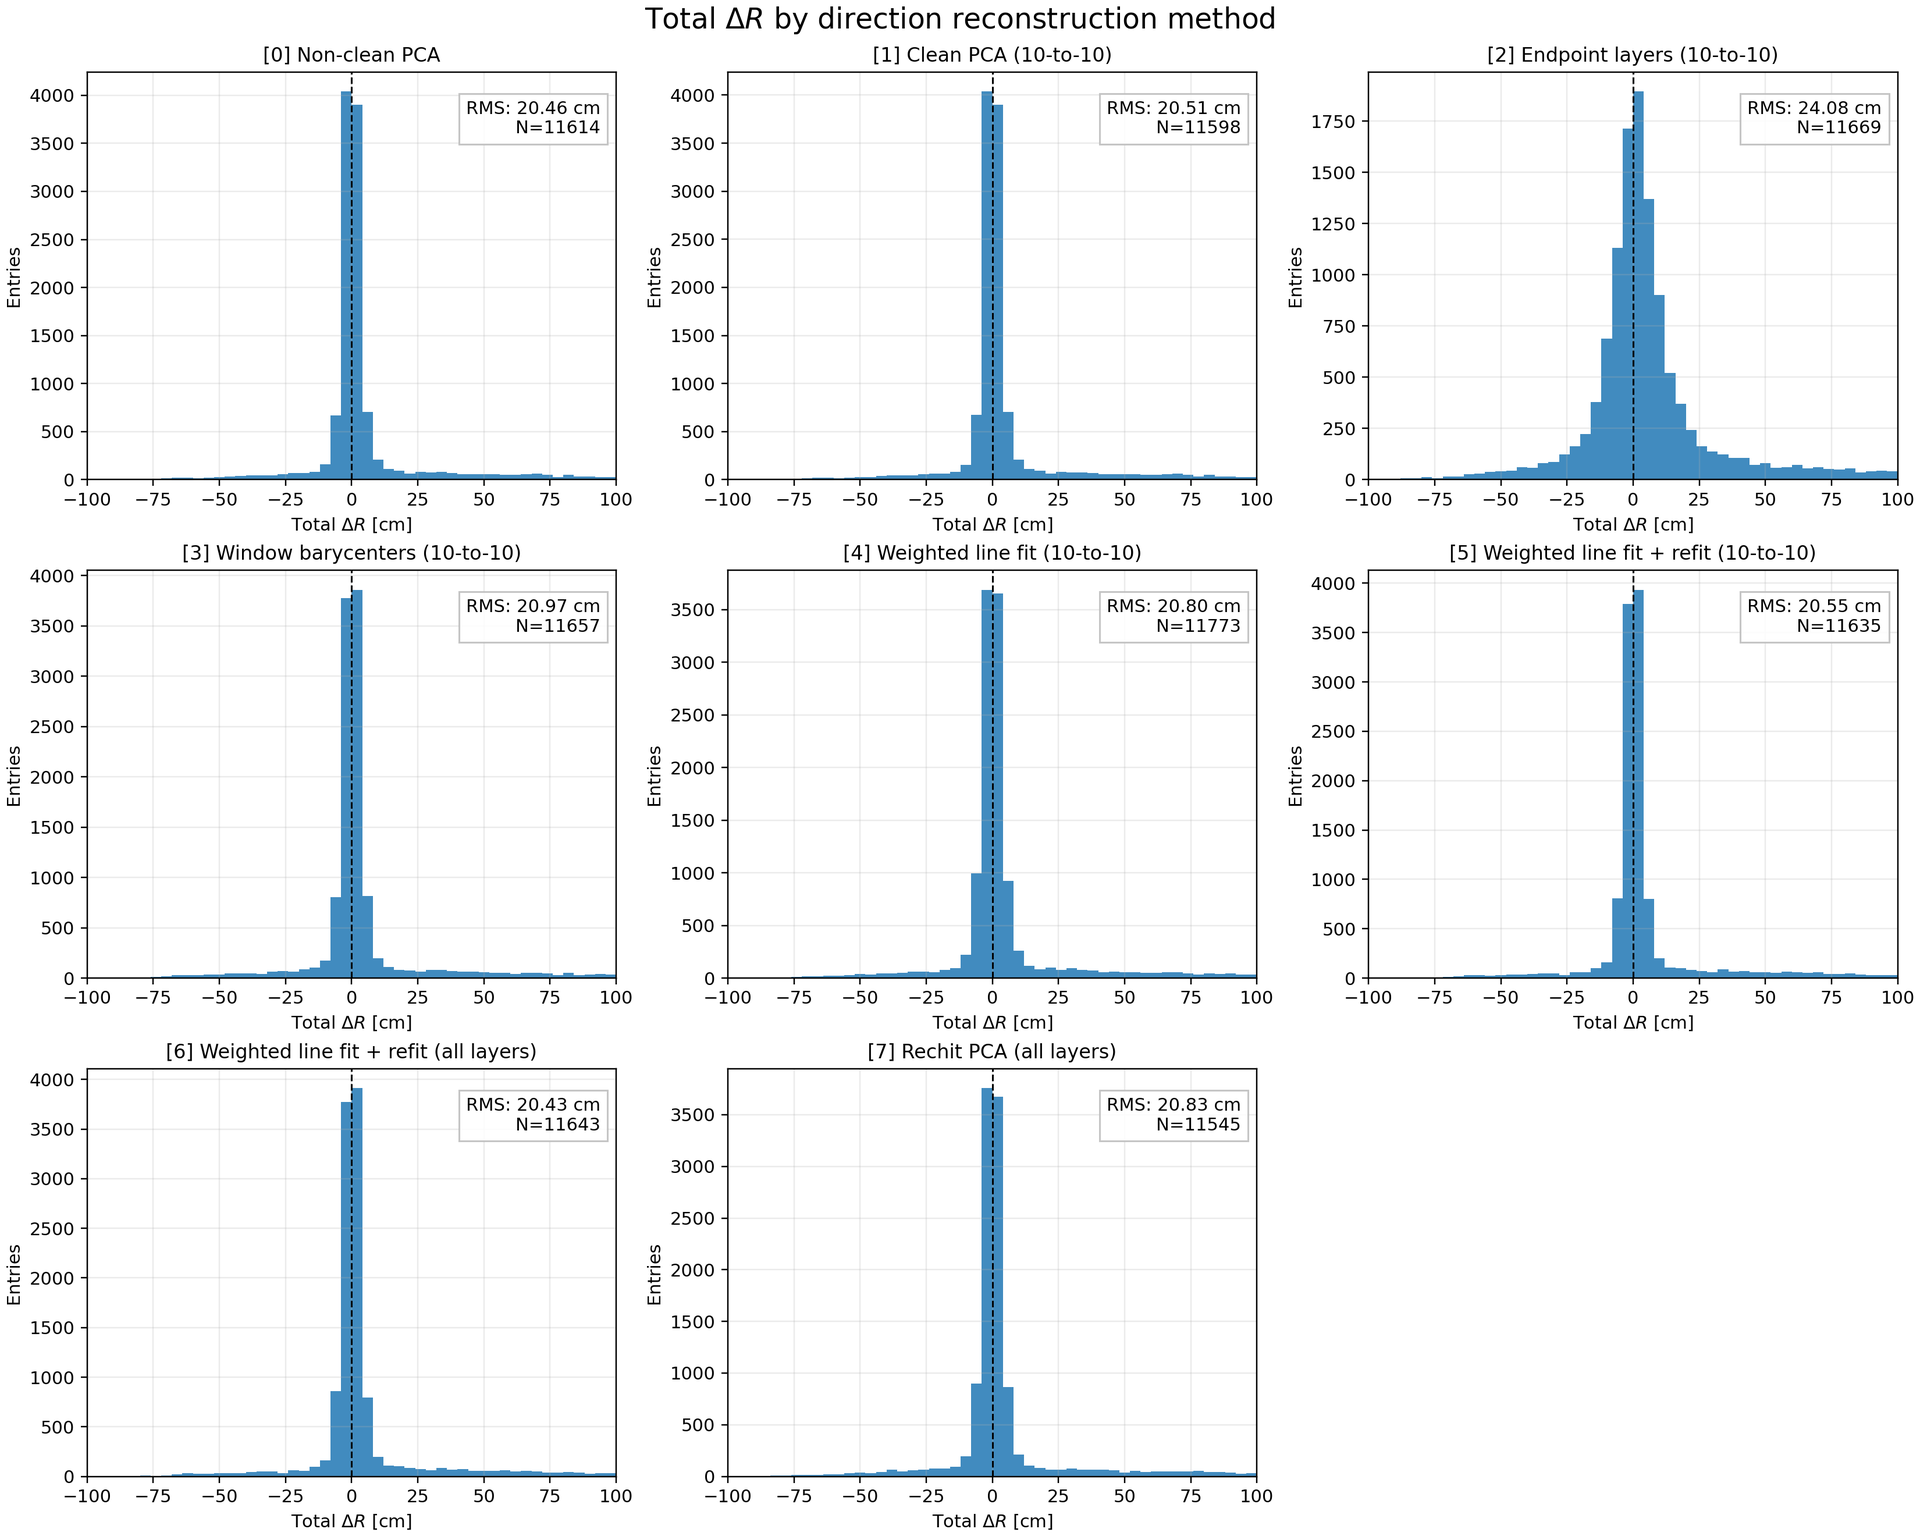
\includegraphics[width=\linewidth]{figures/method_grid_all_tracksters.png}
    \caption{all Tracksters in the event}
    \label{fig:methods-all}
  \end{subfigure}
  \caption{Full-error distribution $\Delta\R$ for each of the eight direction
  estimators, (a) restricting to the leading Trackster and (b) over all
  Tracksters. Restricting to the leading Trackster, the PCA variants are the
  narrowest (clean PCA \SI{9.91}{cm}, ordinary \SI{9.98}{cm}) and the endpoint
  estimate the broadest (\SI{16.07}{cm}). Over all Tracksters every estimator
  instead collapses to $\sim\SI{20}{cm}$. The choice of estimator barely
  matters, because the sample is then dominated by low-energy fragments whose
  direction no method can fit.}
  \label{fig:methods}
\end{figure*}

The comparison (Fig.~\ref{fig:methods}) makes clear that no estimator
improves decisively on the default. On the leading Trackster (most energetic one per event, closest to the truth) the PCA variants are
already the best and the more elaborate line fits merely match them; over all
Tracksters (which includes small fragments) every method collapses to the same $\sim\SI{20}{cm}$, so the estimator
is almost irrelevant and it is the Trackster selection that drives the
resolution. Because the clean PCA is both robust and already implemented in
CMSSW, it was adopted as the default.

\begin{figure*}[!tp]
  \centering
  \begin{subfigure}[b]{0.49\textwidth}
    \centering
    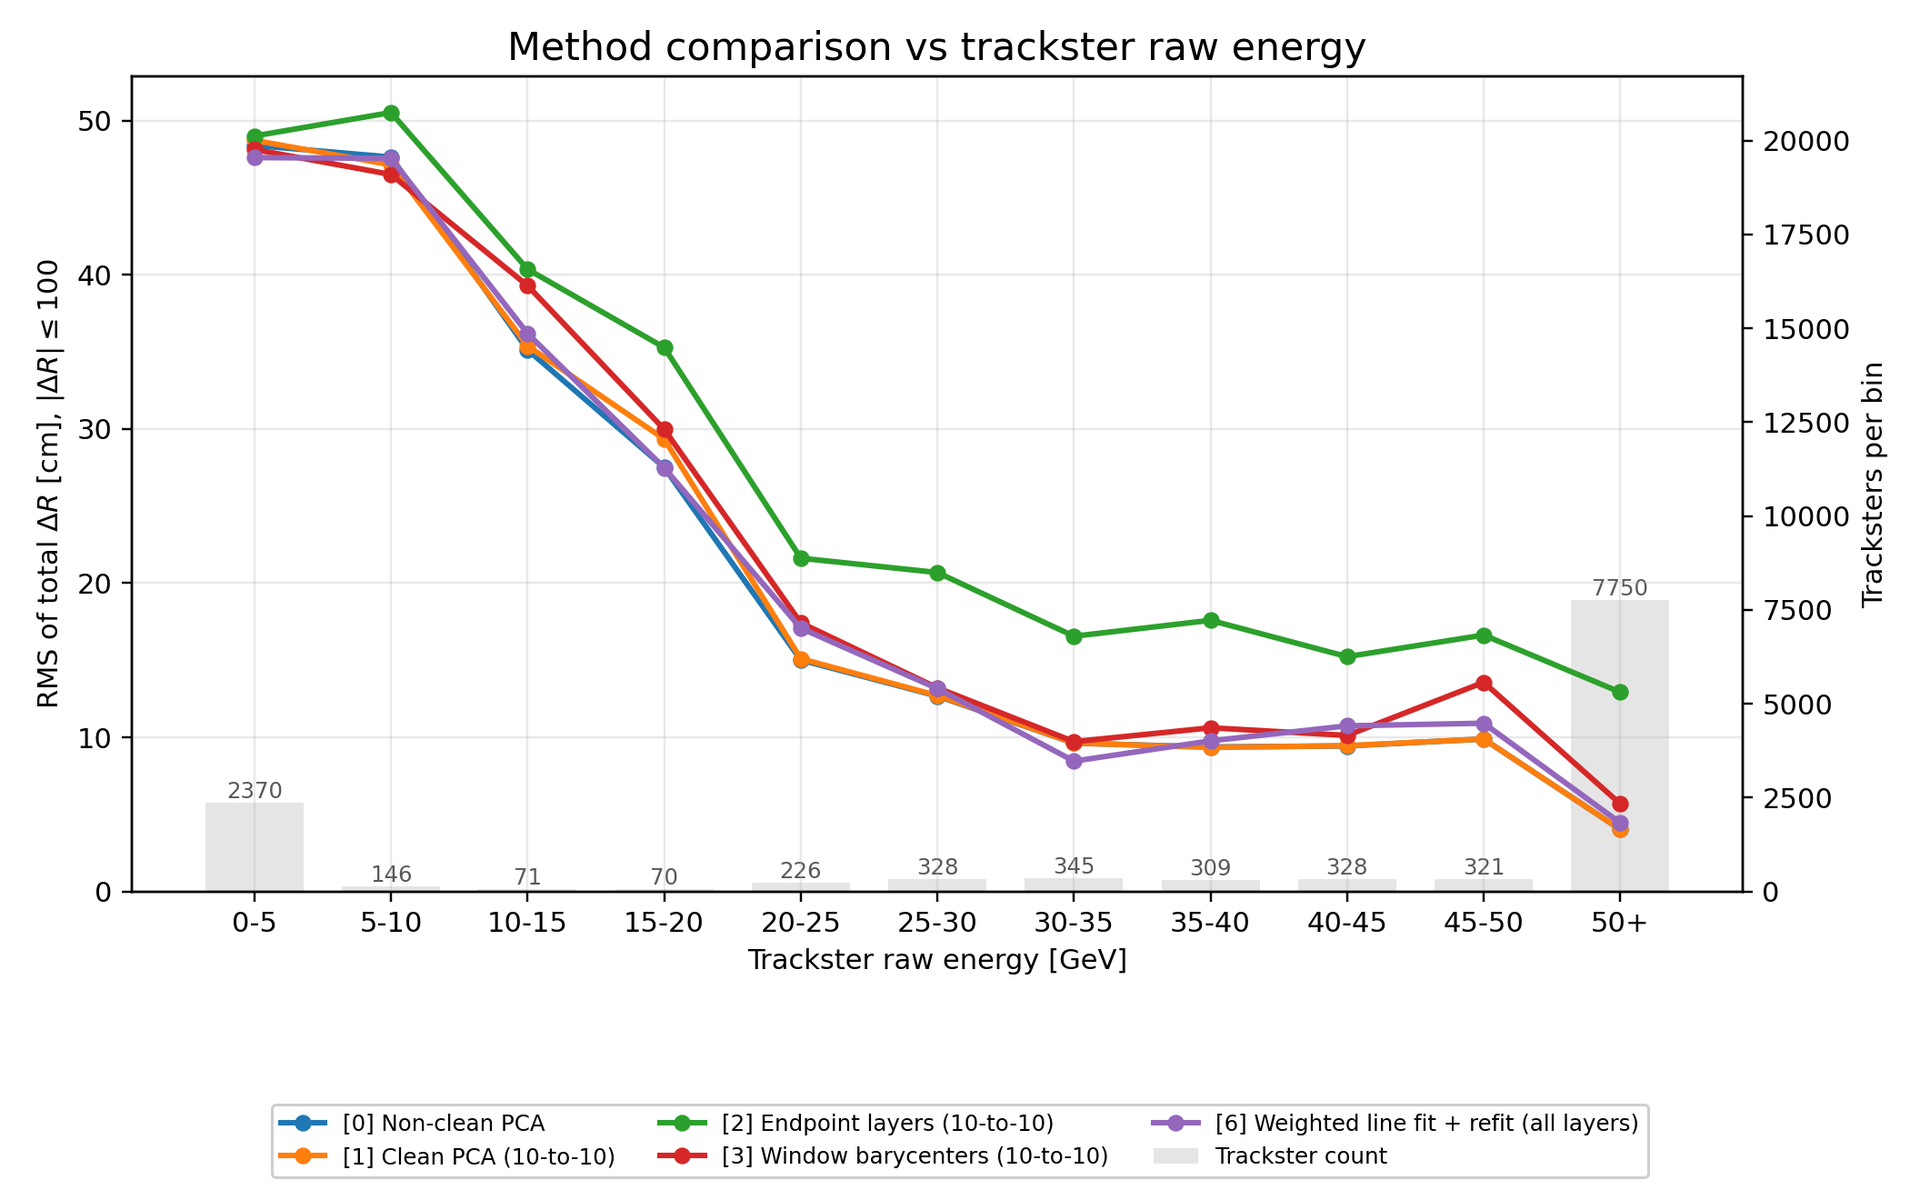
\includegraphics[width=\linewidth]{figures/r_resolution_vs_energy.png}
    \caption{versus Trackster raw energy}
    \label{fig:restrend-e}
  \end{subfigure}
  \hfill
  \begin{subfigure}[b]{0.49\textwidth}
    \centering
    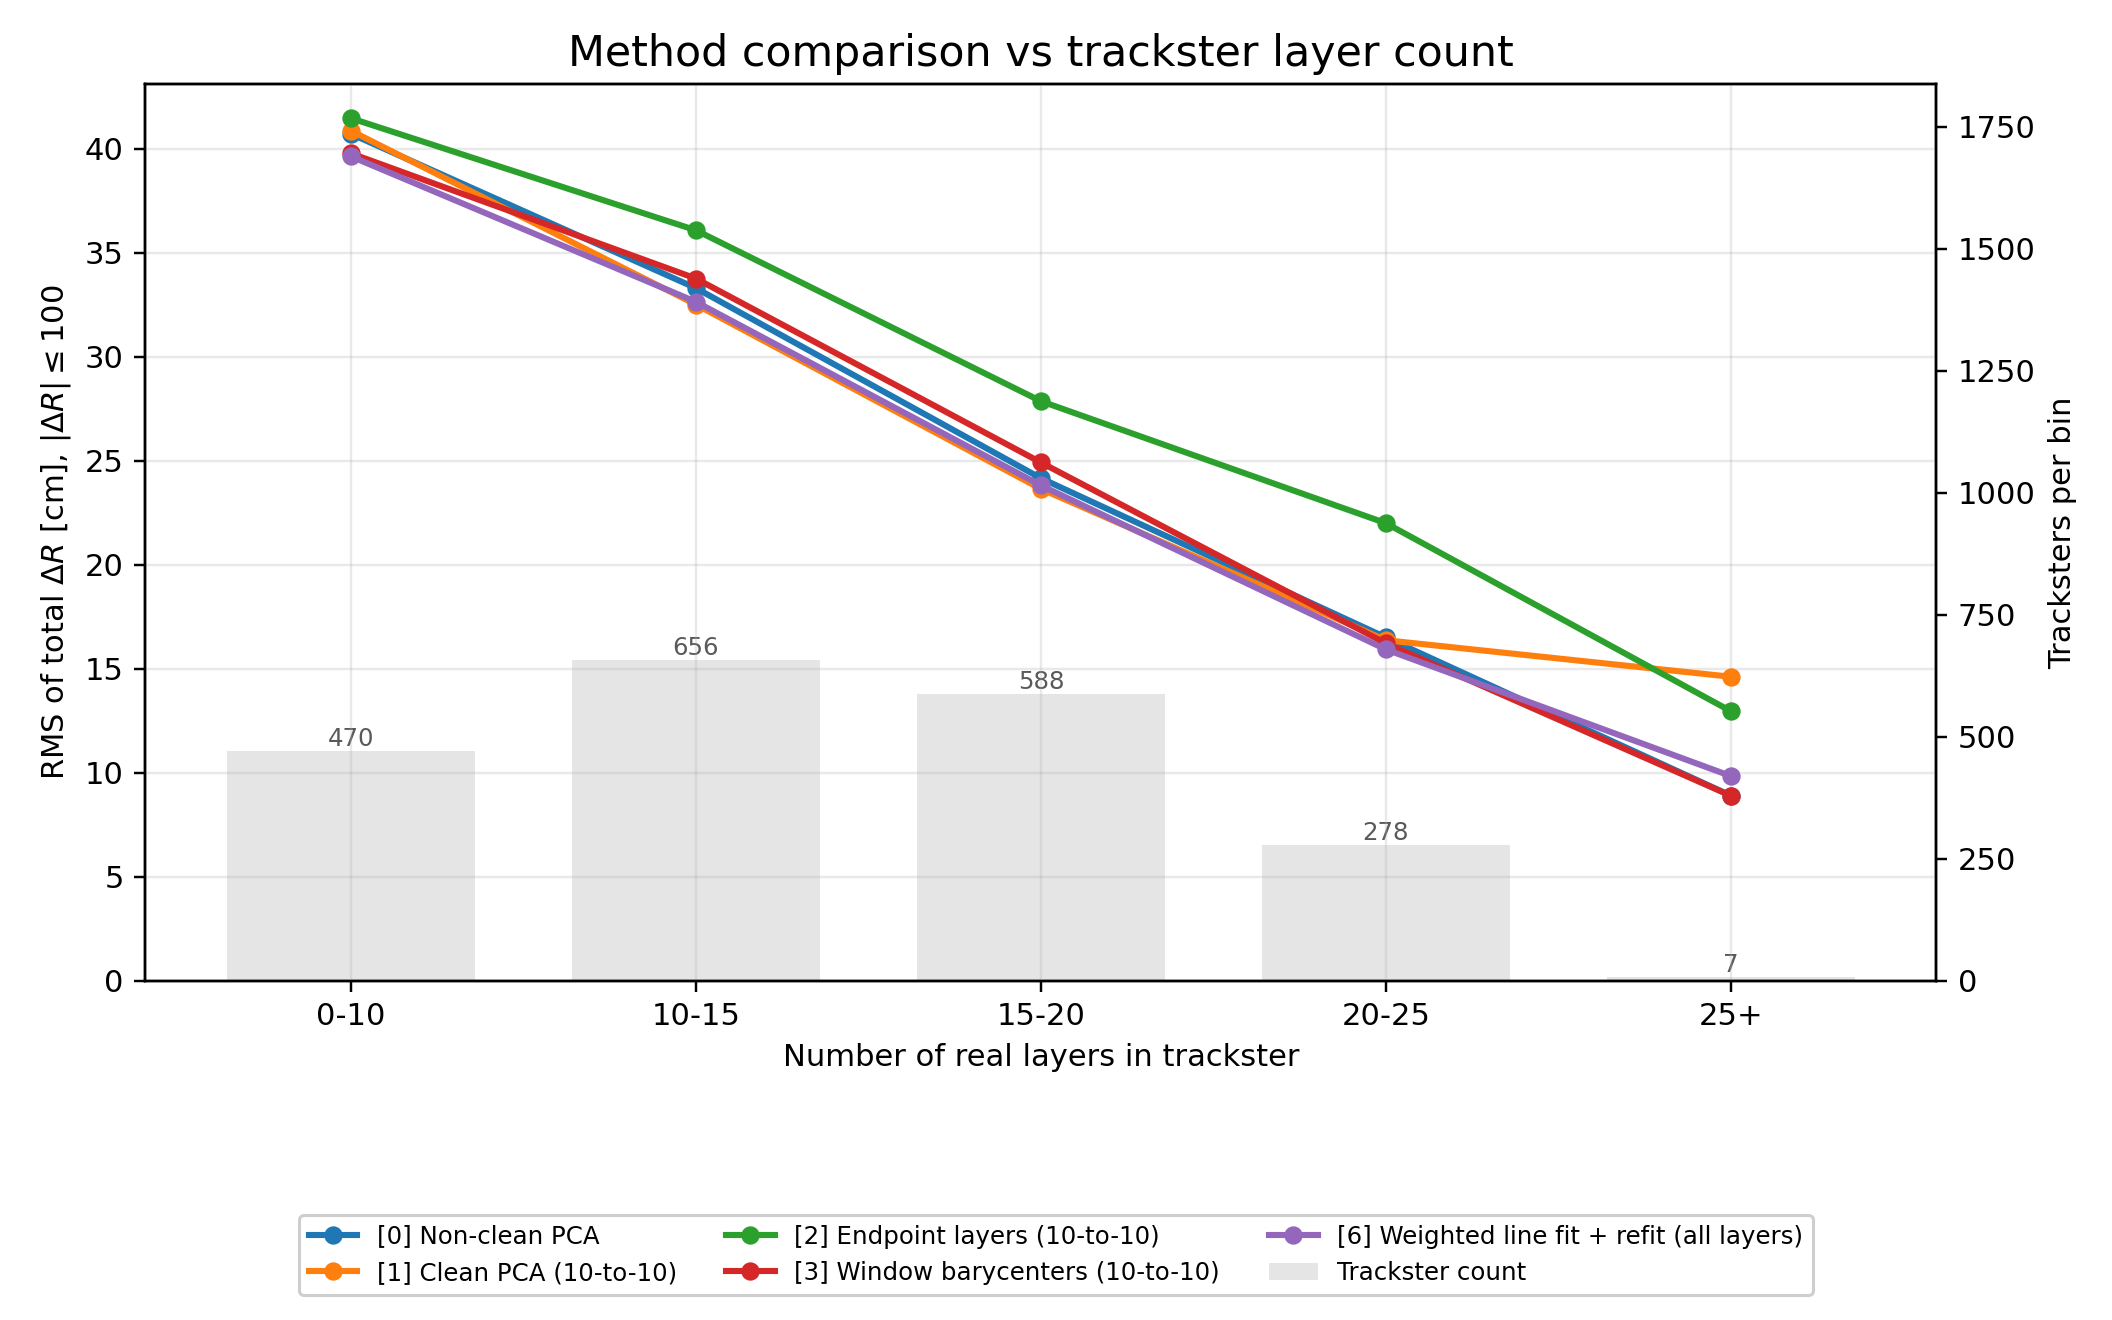
\includegraphics[width=\linewidth]{figures/method_resolution_vs_layer_count.png}
    \caption{versus number of layers}
    \label{fig:restrend-l}
  \end{subfigure}
  \caption{Displacement-radius resolution $\text{RMS}(\Delta\R)$ versus
  (a) Trackster raw energy and (b) the number of layers the Trackster spans, for
  each estimator (coloured curves). The resolution improves by a factor of
  several from low to high energy and from few to many layers, confirming that
  the error tracks how well the shower direction can be fitted. Grey bars (right
  axis) give the Trackster count per bin.}
  \label{fig:restrend}
\end{figure*}

This picture is confirmed by binning the resolution in Trackster observables
(Fig.~\ref{fig:restrend}): the RMS falls from
$\sim\SI{48}{cm}$ below \SI{10}{GeV} to $\sim\SI{10}{cm}$ above \SI{25}{GeV}, and
from $\sim\SI{40}{cm}$ below ten layers to $\lesssim\SI{10}{cm}$ beyond twenty,
with the layer count the cleanest single predictor. The error is thus worst
exactly where the axis is hardest to fit---sparse, low-energy Tracksters spanning
few layers---which is why selecting the single most energetic Trackster per
event, the object that actually carries the photon, is what brings the clean
$10$-to-$10$ PCA to $\text{RMS}(\Delta\R)=\SI{9.91}{cm}$.

We judged this $\sim\SI{10}{cm}$ leading-Trackster resolution good enough to bin
every reconstruction-side metric that follows, and chose the clean $10$-to-$10$
PCA to compute \R{}. A natural next step, left outside the scope of this project,
would be to add a further dimension to the direction fit: each LayerCluster also
carries a timing measurement, and a displaced, non-pointing shower arrives with a
time-of-flight pattern that constrains its direction independently of the spatial
axis. Exploiting Trackster timing to sharpen $\R_{\text{reco}}$ is a promising
avenue for future work.

The displacement observables \R{} and \alphainc{}, together with a
Trackster-timing observable, were added to the standard HGCAL validation as new
per-object quantities so that any efficiency, purity, duplicate or merge plot
can be produced as a function of displacement (CMSSW pull request
\href{https://github.com/cms-sw/cmssw/pull/51510}{\#51510}).
